\section{Reservoir Construction Details}
\label{app:reservoir}

\subsection{Ground-truth filtering criteria}

The initial candidate pool contains more than 800 symbolic regression tasks collected from heterogeneous benchmark families and equation-discovery sources. A task is retained in the ground-truth reservoir only if it satisfies the following evaluation-readiness criteria:
\begin{itemize}
    \item a ground-truth formula is available;
    \item the formula is parsable into a symbolic expression tree;
    \item all variables, constants, and operators are resolvable;
    \item the expression can be executed as a numerical program;
    \item fixed train, ID test, and OOD test splits are available or can be deterministically generated;
    \item target values are finite on all official splits;
    \item the expression variable signature matches the dataset columns;
    \item metadata is sufficient for provenance, structural auditing, and duplicate control.
\end{itemize}

Tasks are removed if they have missing or ambiguous ground-truth formulas, unparsable expressions, unresolved variables, invalid operators, non-finite targets, inconsistent stored targets, missing official splits, or insufficient metadata. After filtering, the ground-truth reservoir contains $|D_{\mathrm{GT}}| = 664$ tasks.

\subsection{Reservoir composition}

After applying the ground-truth filtering criteria, the retained tasks are audited to verify that the reservoir has not collapsed into a narrow subset of formulas or source families. This audit summarizes the 664-task \reservoir{} from both provenance and structural perspectives, including source family, operator usage, formula complexity, and probe-derived difficulty bins.

\begin{figure}[p]
\centering
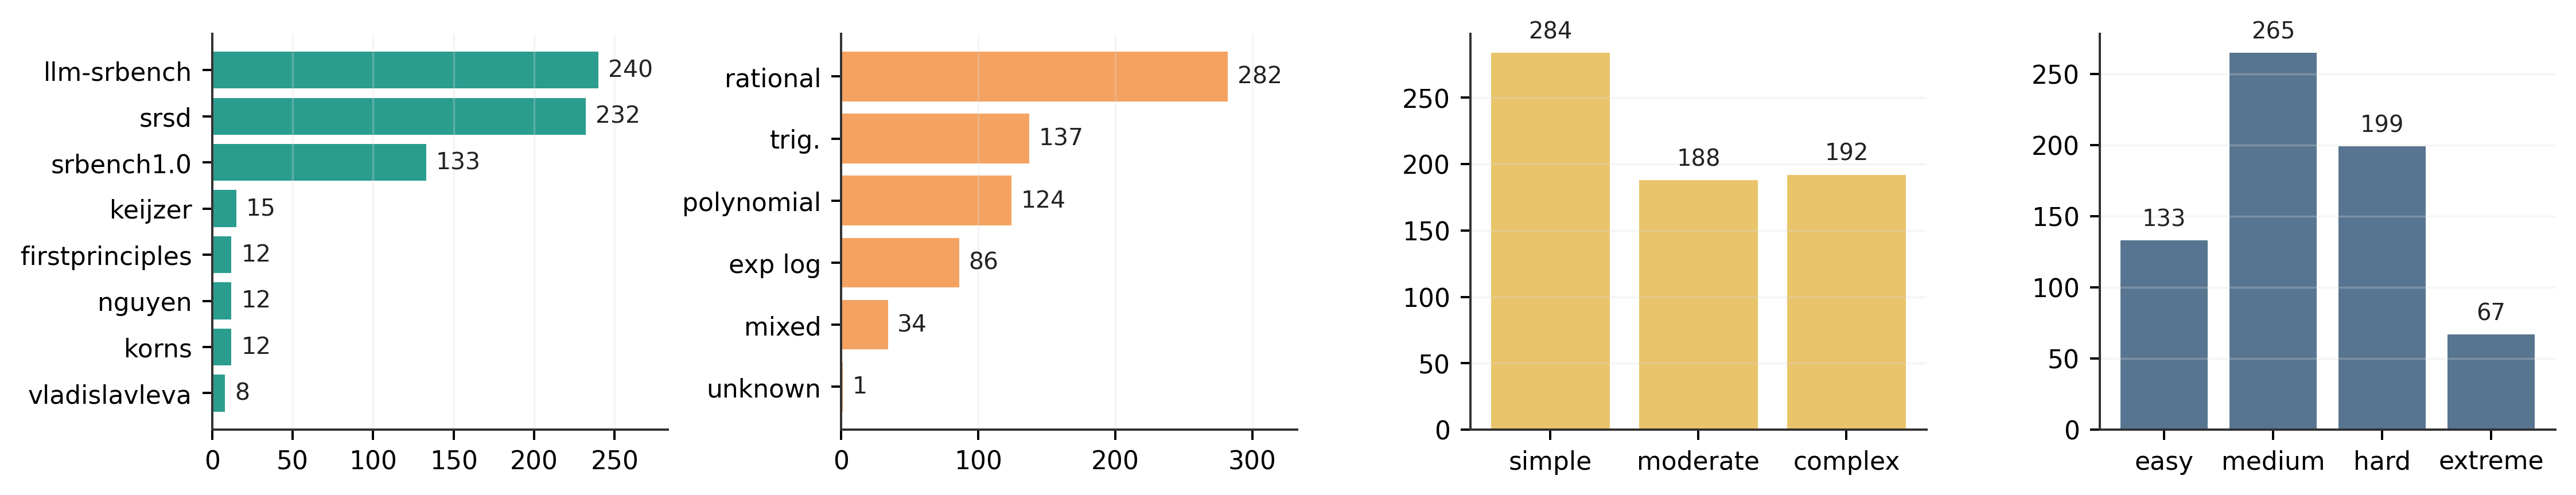
\includegraphics[width=0.88\linewidth]{imgs/Article/figure02_reservoir_composition}
\caption{\textbf{\reservoir{} composition after ground-truth filtering.} The 664-task reservoir retains heterogeneous source families, operator profiles, formula complexities, and probe-derived difficulty bins.}
\label{fig:appendix-reservoir-composition}
\end{figure}

As shown in \cref{fig:appendix-reservoir-composition}, the filtered reservoir remains heterogeneous across dataset provenance, symbolic structure, and empirical difficulty. These composition statistics are used to document the parent task population represented by \core{}, while the actual core-set selection procedure is described separately in the main text.


\subsection{Unified task schema}

Each retained task is stored with a unified schema. The core fields are summarized in \cref{tab:reservoir-schema}.

\begin{table}[t]
\centering
\caption{\textbf{Core fields stored for each task in the ground-truth reservoir.}}
\label{tab:reservoir-schema}
\begin{tabular}{ll}
\toprule
Field & Description \\
\midrule
\texttt{dataset\_id} & Unique task identifier \\
\texttt{family} & Source family or benchmark family \\
\texttt{subgroup} & Sub-family, variant, or task group \\
\texttt{basename} & Original equation or task name \\
\texttt{source\_benchmark} & Original source benchmark \\
\texttt{ground\_truth\_formula} & Raw ground-truth expression \\
\texttt{canonical\_formula} & Canonicalized expression \\
\texttt{train\_split} & Training samples \\
\texttt{id\_test\_split} & In-distribution test samples \\
\texttt{ood\_test\_split} & Out-of-distribution test samples \\
\texttt{n\_features} & Number of input variables \\
\texttt{sample\_count} & Number of samples in each split \\
\texttt{formula\_complexity} & Expression complexity score \\
\texttt{operator\_types} & Operators appearing in the formula \\
\texttt{ood\_type} & Type of OOD split \\
\texttt{dummy\_variable\_flag} & Whether dummy variables are present \\
\texttt{semantic\_duplicate\_group} & Duplicate-control group identifier \\
\bottomrule
\end{tabular}
\end{table}

\subsection{Expression canonicalization}

All ground-truth formulas are converted into a unified symbolic representation. The canonicalization procedure standardizes variable names, operator names, constant formatting, commutative ordering, and expression-tree serialization. For each formula, the following representations are stored:
\begin{itemize}
    \item canonical expression string;
    \item prefix and postfix forms;
    \item expression tree;
    \item operator-normalized form;
    \item constant-normalized form;
    \item Newick-like tree serialization;
    \item canonical skeleton for duplicate and structural-consistency analysis.
\end{itemize}

The raw source expression is also retained to preserve provenance. The canonical representation is used for symbolic equivalence testing, expression-tree comparison, operator and variable recovery, duplicate detection, and seed-level structural consistency in the leaderboard evaluation.

\subsection{Train, ID, and OOD splits}

Each retained task contains fixed train, ID test, and OOD test splits. The training split is used by algorithms during expression search. The ID test split evaluates same-distribution generalization, while the OOD test split evaluates whether the discovered expression extrapolates beyond the training distribution.

If a source benchmark provides compatible official splits, those splits are preserved. Otherwise, splits are deterministically generated from the executable ground-truth program and recorded in the task metadata. Official numerical scores are computed only on the fixed ID and OOD test splits.

\subsection{Quality-control checks}

The following checks are applied before a task enters the reservoir:
\begin{itemize}
    \item expression parsing succeeds;
    \item executable ground-truth program produces finite values on all official splits;
    \item stored targets match executable ground-truth outputs within numerical tolerance;
    \item variable signatures match dataset columns;
    \item canonicalization is deterministic;
    \item required metadata fields are present;
    \item duplicate identifiers and ambiguous records are resolved.
\end{itemize}

These checks ensure that the 664-task reservoir is not merely a collection of regression tables, but a standardized and executable substrate for numerical evaluation, symbolic comparison, and later leaderboard analysis.
